\documentclass[12pt]{article}

% --- Preamble ---
\usepackage[utf8]{inputenc}
\usepackage[english]{babel}
\usepackage{amsmath, amssymb} % For math and symbols
\usepackage{graphicx}
\usepackage{booktabs} % For professional tables
\usepackage{geometry}
\geometry{margin=1in}
\usepackage{hyperref}
\hypersetup{
    colorlinks=true,       % Enables colored links instead of boxes
    linkcolor=blue,        % Color for internal links (sections, figures)
    citecolor=blue,        % Color for bibliographic references
    filecolor=magenta,     % Color for file links
    urlcolor=cyan,         % Color for external URLs
    pdftitle={Satellite-Based Change Detection Implementation}
}
\usepackage[backend=biber, style=authoryear]{biblatex}
\addbibresource{references.bib}

% --- Project Metadata ---
\title{Midterm Project: A Nice Title for your Midterm Project}
\author{Your names}
\date{\today}

\begin{document}

\maketitle

\section{Introduction}
Write down a nice introduction for your project...

\section{Region of Interest (ROI) and Case Study}
Provide a succinct geographic description of the selected event...

\section{Methodology}
Explain your implementation step by step:  The implementation follows a structured five-phase workflow \parencite{Lillesand2015}...

\subsection{Phase 1: Problem Definition \& Data Acquisition}
\begin{itemize}
    \item \textbf{Dates:} Before ($t_1$) and After ($t_2$) selection.
    \item \textbf{Data Sources:} Optical (Sentinel-2 or Landsat 8/9) and/or optional SAR (Sentinel-1).
\end{itemize}

\subsection{Phase 2: Pre-processing}
To ensure images are radiometrically comparable, the following steps were applied:
\begin{itemize}
    \item \textbf{Atmospheric Correction:} \ldots
    \item \textbf{Co-registration:} \ldots
    \item \textbf{Resampling:}  (if needed) \ldots
    \item \textbf{Cloud Masking:} \ldots
\end{itemize}

\subsection{Phase 3: Image Processing \& Analysis}
We utilized specific methods based on the event type.  Table \ref{tab:techniques} show those techniques.

\begin{table}[ht]
    \centering
    \caption{Applied Change Detection Methodologies}
    \label{tab:techniques}
    \begin{tabular}{lll}
        \toprule
        \textbf{Method} & \textbf{Technique} \\
        \midrule
        \ldots & \ldots \\
        \ldots & \ldots \\
        \bottomrule
    \end{tabular}
\end{table}

\subsection{Phase 4: Post-Processing \& Accuracy Assessment}
\begin{itemize}
    \item \textbf{Thresholding:} \ldots
    \item \textbf{Validation:} \ldots
    \item \textbf{Vectorization:} See QGIS details in Figure \ref{fig:vectorization} \parencite{QGIS_Software} \ldots
\end{itemize}

\begin{figure}
 \centering
 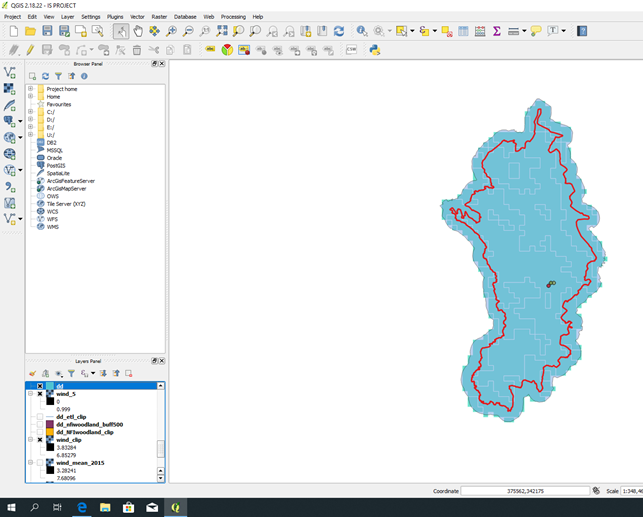
\includegraphics{figures/vectorization}
 \caption{An example of vectorization in QGIS}
 \label{fig:vectorization}
\end{figure}


\section{Results and Discussion}

\subsection{Thematic Maps}
\ldots

\subsection{Statistics:}
\ldots

\subsection{Storytelling \& Discussion}
\ldots

\section{Conclusion}
Write down a nice set of conclusions for this project.

% Print the bibliography here
\printbibliography

\end{document}
